\section{Das Rosenblatt-Perzeptron}\label{sec:rosenblattperceptron}

MCP-Netze sind durch vorhergehende Analyse der Anforderungen und entsprechender Anpassung der Topologie zur Lösung verschiedener Aufgaben imstande. \textit{Donald Hebbs} Theorien über \textit{synaptische Plastizität} führen einige Jahre nach dem MCP-Neuron zu einem Modell, das in der Lage ist, sich selbst anzupassen.


\subsection{Das Perzeptron - ein linearer Klassifizierer}

Bereits 1954 wurden Versuche unternommen, lernfähige neuronale Netze zu modellieren (vgl.~\cite[24]{Ros62}).
1958 schafft es ein Modell, für Aufsehen zu sorgen: Das \textbf{Perceptron} (im folgenden Perzeptron) (vgl.~\cite[89]{AR88}).
1957 beschreibt es sein Schöpfer \textit{Frank Rosenblatt} (1928 - 1971) in~\cite{Ros57} als Teil eines internen Forschungsprojektes des \textit{Cornell Aeronautical Labors}.

\subsection{Das Modell}

Rosenblatt definiert das Perzeptron wie folgt\footnote{
    Ausführliche Definitionen aller Zustände, Signale und Funktionen in~\cite[79 - 94]{Ros62}
}:

\blockquote[{\cite[83 ``DEFINITION 17``; Hervorhebung i.O.]{Ros62}}]{
    A \underline{perceptron} is a network of S, A, and R units with a variable interaction matrix \textit{V} which depends on the
    sequence of past activity states of the network.
}

Dabei ähneln die dort erwähnten A-Units als verrechnende Einheiten nicht bloß zufällig der in Abschnitt~\ref{mcp-inputactivfunc} vorgestellten Aktivierungsfunktion: Rosenblatt selber weist darauf hin, dass er sein Modell direkt von dem von McCulloch und Pitts eingeführten Modell ableitet\footnote{
    vgl. auch ``Ein \texit{einfaches Perzeptron} ist eine McCulloch-Pitts-Zelle, die ihre Eingabe gewichtet berechnet.`` in~\cite[57, ``Definition 3.1``; Hervorhebung i.O.]{Roj93}
}.\\

\begin{figure}[h]
    \begin{center}
        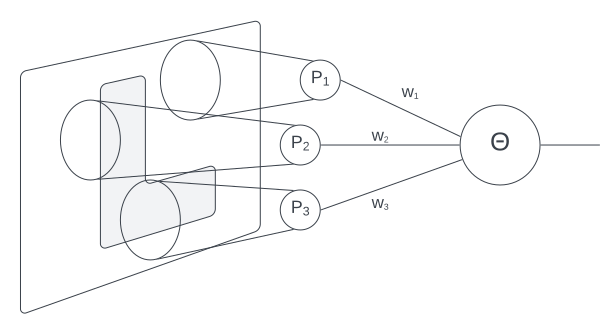
\includegraphics{chapters/3. Kuenstliche Neuronen/images/perzeptron}
        \caption{
            Rosenblatt-Perzeptron. (Quelle: in Anlehnung an~\cite[53, Abb. 3.2]{Roj93})
        }
        \label{fig:perctheda}
    \end{center}
    \small{
        Schematische Darstellung eines Perzeptron-``Automats`` (siehe~\cite[7]{Ros57}): Eingaben werden an die Prädikate $P_n$ weitergeleitet, deren binäre Ausgaben mit den Gewichten $w_n$ multipliziert werden. Die Summe der Produkte wird mit dem Schwellenwert $\Theta$ verglichen (vgl.~\cite[53]{Roj93}).
    }
\end{figure}

\textit{Rojas} schreibt, dass das klassische Rosenblatt-Perzeptron in einem Netz von Eingabe- und Ausgabeknoten gewichtete Verbindungen nutzt - die Knoten selber sind Schwellenwertelemente, Verbindungen werden stochastisch ermittelt (siehe~\cite[51]{Roj93}).
Er weist ebenda darauf hin, dass das Modell nach Rosenblatts Veröffentlichung analysiert und verfeinert wurde, u. a. von \textit{Minsky und Papert} in~\cite{MP88}, die wie folgt definieren:

\blockquote[{\cite[12; Hervorhebung i.O.]{MP88}}]{
    A \underline{perceptron} is a device capable of computing all predicates which are linear in some given set $\Phi$ of partial predicates.
}

\textit{Prädikate} sind hier Verbindungen zu den Eingabesignalen, die einen Wahrheitswert $0$ oder $1$ basierend auf der Eingabe $X$ berechnen.
Die Ausgaben der Prädikate werden individuell gewichtet und an die Zelle weitergeleitet, die die Aktivierungsfunktion implementiert (vgl.~\cite[52 f.]{Roj93} und~\cite[8-12]{MP88}).

Diese Eingabefunktion setzt sich wie Gleichung~\ref{eq:gl-mcpinpfunc} aus der Summe der Produkte der Prädikate $P_i \in \Phi$ (wobei $P_i(X) \in \{0, 1\}$) und den Gewichten $w_i \in \mathbb{R}$ der Verbindungen zusammen (s. Gleichung~\ref{eq:gl-rpinput}), und die Aktivierungsfunktion (s. Gleichung~\ref{eq:gl-rpact}) ist wieder eine Treppenfunktion mit dem reellen Schwellenwert $\Theta$:

\begin{equation}
g \coloneqq g(X) = \sum^n_{i=1} P_i(X) w_i
\label{eq:gl-rpinput}
\end{equation}

\begin{equation}
    f \coloneqq f(g(X)) = f(x) = \begin{cases}
                          1 \text{ falls } x >= \Theta \\
                          0 \text{ falls } x < \Theta
\end{cases}
\label{eq:gl-rpact}
\end{equation}


\subsection{Lineare Trennbarkeit}
Mit Gleichung~\ref{eq:gl-rpact} folgt für eine Eingabe, dass sie entweder eine $0$ oder $1$ als Ausgabe erzeugt.
Es liegt ein binärer Wertebereich vor, der als zwei unterschiedliche Klassen aufgefasst werden kann: Eingabedaten können entsprechend ihrer Ausgabe einer der beiden Klassen zugeordnet werden (vgl.~\cite[812]{RN09}).
Im Folgenden sollen die Zusammenhänge geometrisch dargestellt werden.
Der Einfachheit halber beschränken wir uns hierzu auf den zweidimensionalen Raum $\mathbb{R}^2$ und betrachten dort die \textit{1. Winkelhalbierende} im I. und III. Quadranten des kartesischen Koordinatensystems.
Die zugehörige \textit{Gerade} $L$ ist

\begin{equation}
L = \{(x_1, x_2) \in \mathbb{R}^2: x_1 = x_2\}
\end{equation}


\begin{figure}[h]
    \centering
    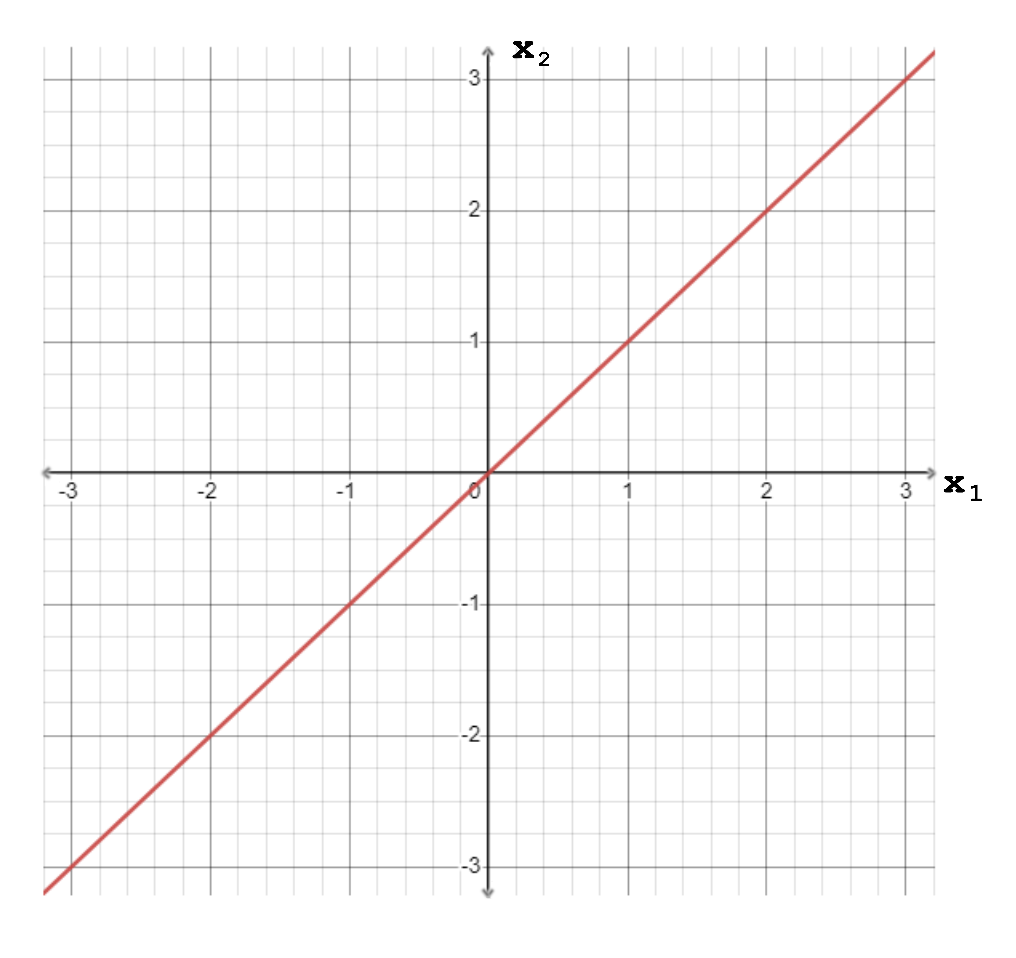
\includegraphics[
        width=12cm,
        keepaspectratio,
    ]{chapters/3. Kuenstliche Neuronen/images/winkelhalbierende}
    \caption{1. Winkelhalbierende im kartesischen Koordinatensystem (Quelle: Eigene Darstellung)}
    \label{fig:winkelhalbierende}
\end{figure}

Für beliebige Punkte $(x_1, x_2) \in \mathbb{R}^2$ gilt damit offensichtlich

\begin{equation}
x_1 - x_2 \begin{cases}
               > 0 \text{ falls } x_1 > x_2 \\
               = 0 \text{ falls } x_1 = x_2 \\
               < 0 \text{ falls } x_1 < x_2
\end{cases}
\end{equation}

Die \textit{Gerade} $L$ repräsentiert eine \textit{Hyperebene}\footnote{
    siehe~\cite[81, Definition 2.3]{BHW+12}
} im $\mathbb{R}^2$.
Punkte, die nicht zu dieser Hyperebene gehören, liegen in zwei unterschiedlichen \textit{Halbräumen} (siehe geometrische Darstellung in Abbildung~\ref{fig:halbraeume}).

Wir können feststellen, dass


\begin{itemize}
    \item Punkte, die $x_1 - x_2 > 0$ erfüllen (im folgenden $M_-$) in dem Halbraum \textit{unter} der durch $L$ beschriebenen Gerade liegen
    \item Punkte, für die  $x_1 - x_2 < 0$ gilt (im folgenden $M_+$) \textit{über} der durch $L$ beschriebenen Gerade liegen
    \item Punkte mit $x_1 - x_2 = 0$ \textit{auf} der Geraden liegen (im folgenden als Teilmenge von $M_-$)
\end{itemize}


\begin{figure}[h]
    \begin{center}
    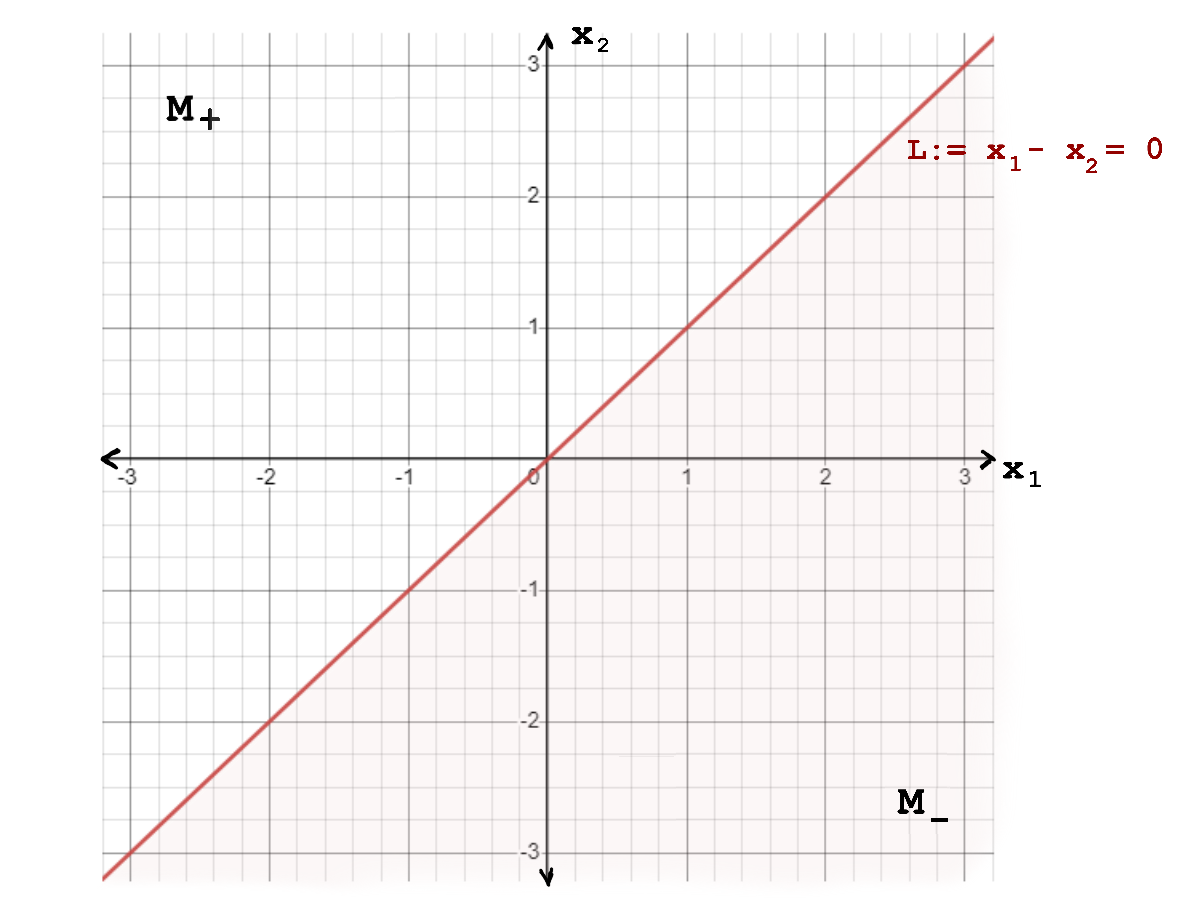
\includegraphics[
        width=12cm,
        keepaspectratio,
    ]{chapters/3. Kuenstliche Neuronen/images/halbraum}
    \caption{Halbräume im $R^2$ (Quelle: Eigene Darstellung)}
    \label{fig:halbraeume}
    \end{center}
    \small{
        Skizzierung der durch die 1. Winkelhalbierende entstandenen Halbräume. Die Mengen $M_-$ und $M_+$ sind linear separierbar, die Gleichung für die \textit{Trenngerade} hierzu lautet $x_1 - x_2 = 0$
    }
\end{figure}



$M_+$ und $M_-$ sind damit \textit{linear separierbar}. Nach \textit{Rojas} lautet die Definition für \textbf{Lineare Trennbarkeit}:

\blockquote[{\cite[60 f., ``Definition 3.2``; Hervorhebung i.O.; Nummerierung eigene]{Roj93}}]{
    \noindent
    Zwei Mengen \textit{A} und \textit{B} von Punkten in einem \textit{n}-dimensionalen Raum sind \textit{linear trennbar}, falls \textit{n}+1 reelle Zahlen $w_1, ... , w_{n+1}$ existieren, so dass für jeden Punkt $x_1, ... , x_n \in A$ gilt

    \begin{equation}
        \sum^n_{i=1} w_ix_i \geq w_{n+1}
        \label{eq:gl-defhalbraum-gl1}
    \end{equation}

    und für jeden Punkt $x_1, ... , x_n \in B$

    \begin{equation}
        \sum^n_{i=1} w_ix_i < w_{n+1}
        \label{eq:gl-defhalbraum-gl2}
    \end{equation}
}



\noindent
Insgesamt kann ein Perzeptron als Funktion verstanden werden. \textit{Ertel} definiert hierzu :

\blockquote[{\cite[212, ``Definition 8.3``; Hervorhebung i.O.]{Ert21a}}]{
    \noindent
    Sei $w = (w_1, ..., w_n) \in  \mathbb{R}^n$ ein Gewichtsvektor und $x \in  \mathbb{R}^n$ ein Eingabevektor. Ein \textbf{Perzeptron} stellt eine Funktion $P:  \mathbb{R}^n \to \{0, 1\}$ mit

    \begin{equation}
        \nonumber
        P(x) = \begin{cases}
                   1 \text{ falls } wx = \sum^n_{i=1} w_ix_i >0 \\
                   0 \text{ sonst }
        \end{cases}
    \end{equation}
    \noindent
    dar.
}

\subsection*{Das Bias-Gewicht}
Die sogenannte \textbf{bias unit} ermöglicht eine Trennbarkeit von Punktmengen, die nicht durch eine Ursprungsgerade separierbar sind (siehe Abbildung~\ref{fig:nichtseparierbar}): Das Bias-Gewicht\footnote{
    vgl.~\cite[839]{RN09}
} ist ein Wert, der zu der Gleichung~\ref{eq:gl-rpinput} hinzuaddiert wird.
In der geometrischen Darstellung sorgt dieser Wert für eine Verschiebung der Ursprungsgeraden entlang der $x_2$-Achse\footnote{
    im $ \mathbb{R}^n$ durch eine Hyperebene im Ursprung (vgl.~\cite[215]{Ert21a}).
}.

\begin{figure}[h]
    \centering
    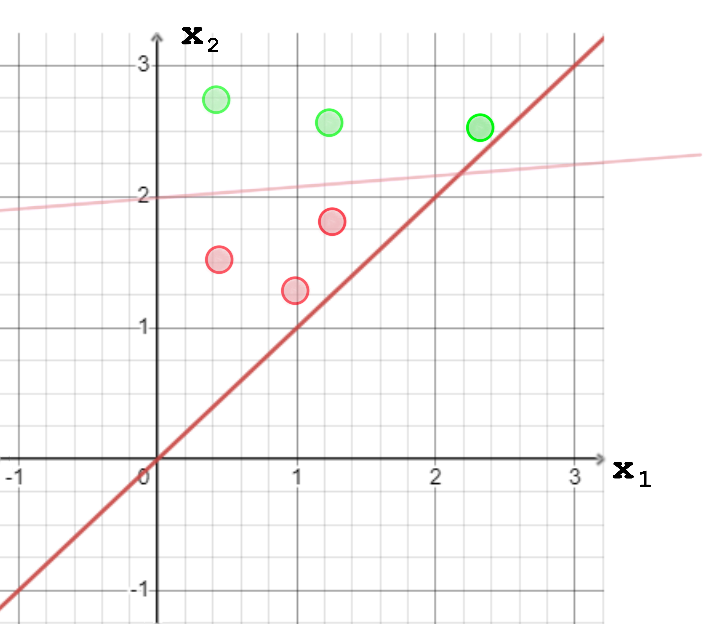
\includegraphics[
        width=8cm,
        keepaspectratio,
    ]{chapters/3. Kuenstliche Neuronen/images/nichtseparierbar}
    \caption{Punkte im $\mathbb{R}^2$, die nicht durch eine Ursprungsgerade separierbar sind. Angedeutet eine mögliche Trenngerade, die durch $(0,2)$ geht. (Quelle: Eigene Darstellung)}
    \label{fig:nichtseparierbar}
\end{figure}


\subsection{Die Lernregel}\label{sec:lernregel}

Die Eigenschaft linearer Trennbarkeit von Daten ist eine wesentliche Voraussetzung dafür, dass ein Perzeptron \textbf{konvergiert}: Die \textbf{Lernregel} des Perzeptrons passt während der Laufzeit die Gewichte $w_1 ... w_n$ solange an, bis sie - eingesetzt in eine lineare Gleichung (vgl.~\cite[311]{Ert21b}) - die $n$-dimensionalen Daten entsprechend Gleichung~\ref{eq:gl-rpact} \textit{klassifizieren} kann.
Aus diesem Grund wird das Perzeptron auch \textbf{linearer Klassifizierer} genannt (vgl.~\cite[210-216]{Ert21a}).

Das Perzeptron \textbf{lernt} diese Gewichte zunächst durch \textit{Trainingsdaten}.
Jeder Eintrag dieser Trainingsdaten ist einer erwarteten Ausgabe zugeordnet. Der Algorithmus besteht aus folgenden Schritten (vgl.~\cite[65]{RM87} sowie~\cite[842]{RN09}):



\begin{enumerate}
    \item Wähle einen Datensatz und berechne die Ausgabe.
    \item Wenn die Ausgabe $1$ ist, obwohl sie $0$ sein sollte (Fehler\footnote{
    Der \textbf{Fehler} ist die Differenz von $\text{erwarteter Ausgabe}$ und $\text{tatsächlicher Ausgabe}$.
    } $=-1$), verringere die Gewichte.
    \item Wenn die Ausgabe $0$ ist, obwohl sie $1$ sein sollte  (Fehler $=1$), erhöhe die Gewichte.
    \item Wenn die Ausgabe korrekt ist, passe die Gewichte nicht an.
\end{enumerate}

\noindent


\noindent
Die Schritte werden so lange durchlaufen, bis für alle Trainingsdaten die Ausgabe korrekt ist, oder eine maximale Anzahl von Trainingsläufen erreicht wurde.
Einen Trainingslauf nennt man dabei \textbf{Epoche}\footnote{siehe ~\cite[436]{Fau94}}.
Sind die Trainingsdaten linear separierbar, {konvergiert}\footnote{
    ``iterative training processes converge if the weight updates reach equilibrium (stop changing)``~\cite[425 ``Convergence``]{Fau94}.
} das Perzeptron nach einer endlichen Zahl von Epochen (vgl.~\cite[164]{MP88})\footnote{
    Das Konvergenz-Theorem besagt: ``if a linear separation exists, the perceptron error-correction scheme will find it.``~\cite[20]{Arb03}. Beweise führen~\cite[111 ff.]{Ros62}, \cite[168 ff.]{MP88} sowie \cite{Nov62}.
}, und ist danach in der Lage weitere Daten zu \textbf{generalisieren} (vgl.~\cite[202]{Ert21a}).\\


\subsection{Die XOR-Funktion}

Wenn ein Perzeptron nicht konvergiert, kann es ausreichen, die Anzahl der Epochen zu erhöhen, damit ein passender Gewichtsvektor gefunden wird (vgl.~\cite[20]{Arb03}).

\begin{figure}[h]
    \begin{center}
    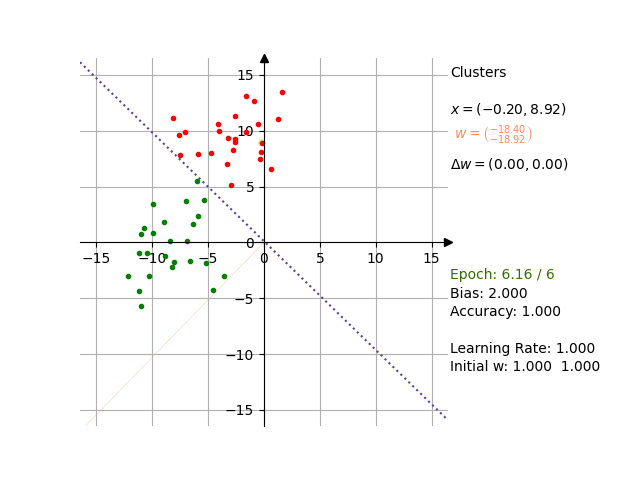
\includegraphics{chapters/3. Kuenstliche Neuronen/images/blob_success}
    \caption{Perzeptron-Training für große Datenmengen. (Quelle: Eigene Darstellung)}
    \label{fig:rp-blobs}
    \end{center}
    \small Ein Perzeptron wird mit einer großen Datenmengen (50 Einträge) trainiert. Nach knapp 300 Trainingsschritten (in der 6ten Epoche) wird die Trenngerade (gestrichelt) gefunden.
\end{figure}

\noindent
Allerdings kann es bereits bei wenigen Daten und beliebig großer Epochenzahl vorkommen, dass ein Perzeptron nicht konvergiert, nämlich wenn die Daten nicht linear separierbar sind (vgl.~\cite[20]{Arb03}).

Als Beispiel betrachten wir die boolesche Funktion \textbf{XOR} (vgl. Tabelle~\ref{tab:xor}).
In Abbildung~\ref{fig:rp-xor} ist die geometrische Repräsentation der möglichen Interpretationen für $A \oplus B$ dargestellt.
Zwar lassen sich die Elemente separieren, aber nicht linear.
Es müsste sonst ein $w_1, w_2$ existieren, das folgende Ungleichungen erfüllt:\\


$w_10 + w_20 < \Theta$\\

$w_11 + w_20 \geq \Theta \implies w_1 \geq \Theta$\\

$w_10 + w_21 \geq \Theta \implies w_2 \geq \Theta$\\

$w_11 + w_21 < \Theta$\\

\noindent
Offensichtlich kann $w_1 + w_2 < \Theta$ nicht erfüllt werden, wenn gleichzeitig $w_1 \geq \Theta$ und $w_2 \geq \Theta$ gilt (s. Abbildung~\ref{fig:rp-xor}).

\begin{figure}[htpb]
    \begin{center}
        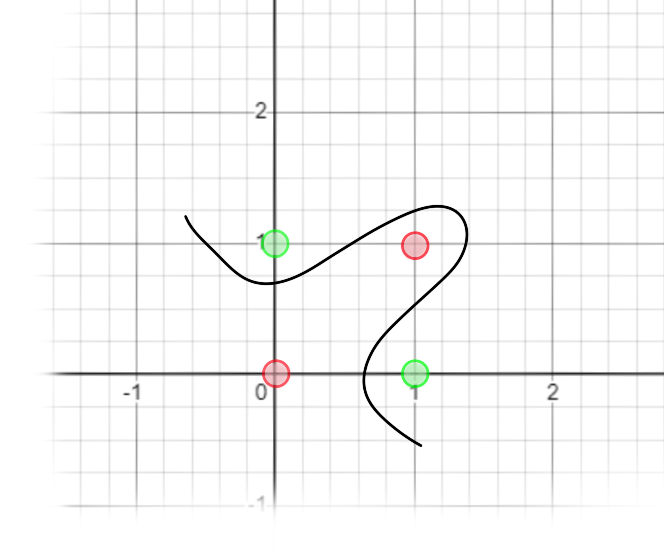
\includegraphics[
            width=8cm,
            keepaspectratio,
        ]{chapters/3. Kuenstliche Neuronen/images/xorr2}
        \caption{XOR im $\mathbb{R}^2$. (Quelle: Eigene Darstellung)}
        \label{fig:rp-xor}
    \end{center}
    \small{
        Interpretationen der XOR-Funktion im kartesischen Koordinatensystem. Hier existiert keine Trenngerade für die Punkte $\{(0, 0), (1, 1)\}$ und $\{(0, 1), (1, 0)\}$.
    }
\end{figure}
